
%%%%%%%%%%%%%%%%%%%%%%%%%%%%%%%%%%%%%%%%%%%%%%%%%%%%%%%%%%%%%%%%%%%%
\section{Organization and Management (David Newbold \& Georgia Karagiorgi)}
\label{sec:fd-daq-org}

%\metainfo{2 Pages}
At the time of writing, the DAQ Consortium comprises 30 institutions, including universities and national labs, from five countries. Ever since its conception, the DAQ Consortium has met roughly on a weekly basis, and has so far held two international workshops dedicated to advancing the DUNE FD DAQ design.

Several key technical and architectural decisions have been made in the last months, that have formed an agreed basis for the DAQ design and implementation presented in this document.

%%%%%%%%%%%%%%%%%%%%%%%%%%%%%%%%%%%
\subsection{DAQ Consortium Organization}
\label{sec:fd-daq-org-consortium}

The DUNE DAQ Consortium is currently organized in the form of five active
Working Groups (WG) and WG Leaders:
\begin{itemize}
\item Architecture, WG Leaders: Giles Barr and Giovanna Lehman-Miotto 
\item Hardware, WG Leaders: David Cussans and Matthew Graham
\item Data Selection, WG Leader: Josh Klein
\item Back-End, WG Leader: Kurt Biery
\item Integration and Infrastructure, WG Leader: Alec Habig
\end{itemize}

During the ongoing early stages of the design, the Architecture and Hardware WGs have been holding additional meetings focused on aspects of the design related to architecture solutions and costing. In parallel, the DAQ Simulation Task Force effort which was in place at the time of the Consortium inception has been adopted under the Data Selection WG, and simulation studies have continued to inform design considerations. This working structure is expected to remain in place through at least the completion of the Technical Proposal. During the construction phase of the project we anticipate a new organisation, built around the major WBS responsibilities.

%%%%%%%%%%%%%%%%%%%%%%%%%%%%%%%%%%
\subsection{Planning Assumptions}
\label{sec:fd-daq-org-assmp}

The DAQ planning is based the assumption of a first single-phase and second dual-phase module. The schedule is sensitive to this assumption, as the DAQ requirements for the two module types are quite different. We plan five partially-overlapping phases of activity (see Fig.~\ref{fig:daq-schedule}):

\begin{itemize}
	\item A further period of R\&D activity, beginning at the time of writing, and culminating in a documented system design in the TDR in July 2019
	\item Production and testing of a full prototype DAQ slice of realistic design, culminating in an Engineering Design Review
	\item Preparation and fit out of the CUC DAQ room with a minimal DAQ slice, in support of the first module construction
	\item Production and delivery of final hardware, computing, software and firmware for the first module
	\item Production and delivery of final hardware, computing, software and firmware for the second module
\end{itemize}

This schedule assumes beneficial occupancy of the CUC DAQ room by end of 22Q1, and the availability of facilities to support an extended large-scale integration test in 2020 (e.g. CERN or FNAL). We assume the availability of resources for installation of final DAQ hardware (e.g. surface control room facilities) from around of 23Q1, and the Integration and Test Facility from 22Q2. Capital resources for DAQ construction will be required from 22Q2, with a first tranche of funds for the minimal DAQ slice from 21Q1.

%%%%%%%%%%%%%%%%%%%%%%%%%%%%%%%%%%%
%\subsection{WBS and Responsibilities}
%\label{sec:fd-daq-org-wbs}

% Apparently this is no longer required? DMN

%%%%%%%%%%%%%%%%%%%%%%%%%%%%%%%%%%
\subsection{High-level Cost and Schedule}
\label{sec:fd-daq-org-cs}

The high-level DAQ schedule, which is compatible with the current DUNE FD top-level schedule is shown in Fig.~\ref{fig:daq-schedule}.

\begin{dunefigure}[DAQ high-level schedule]{fig:daq-schedule}
  {DAQ high-level schedule}
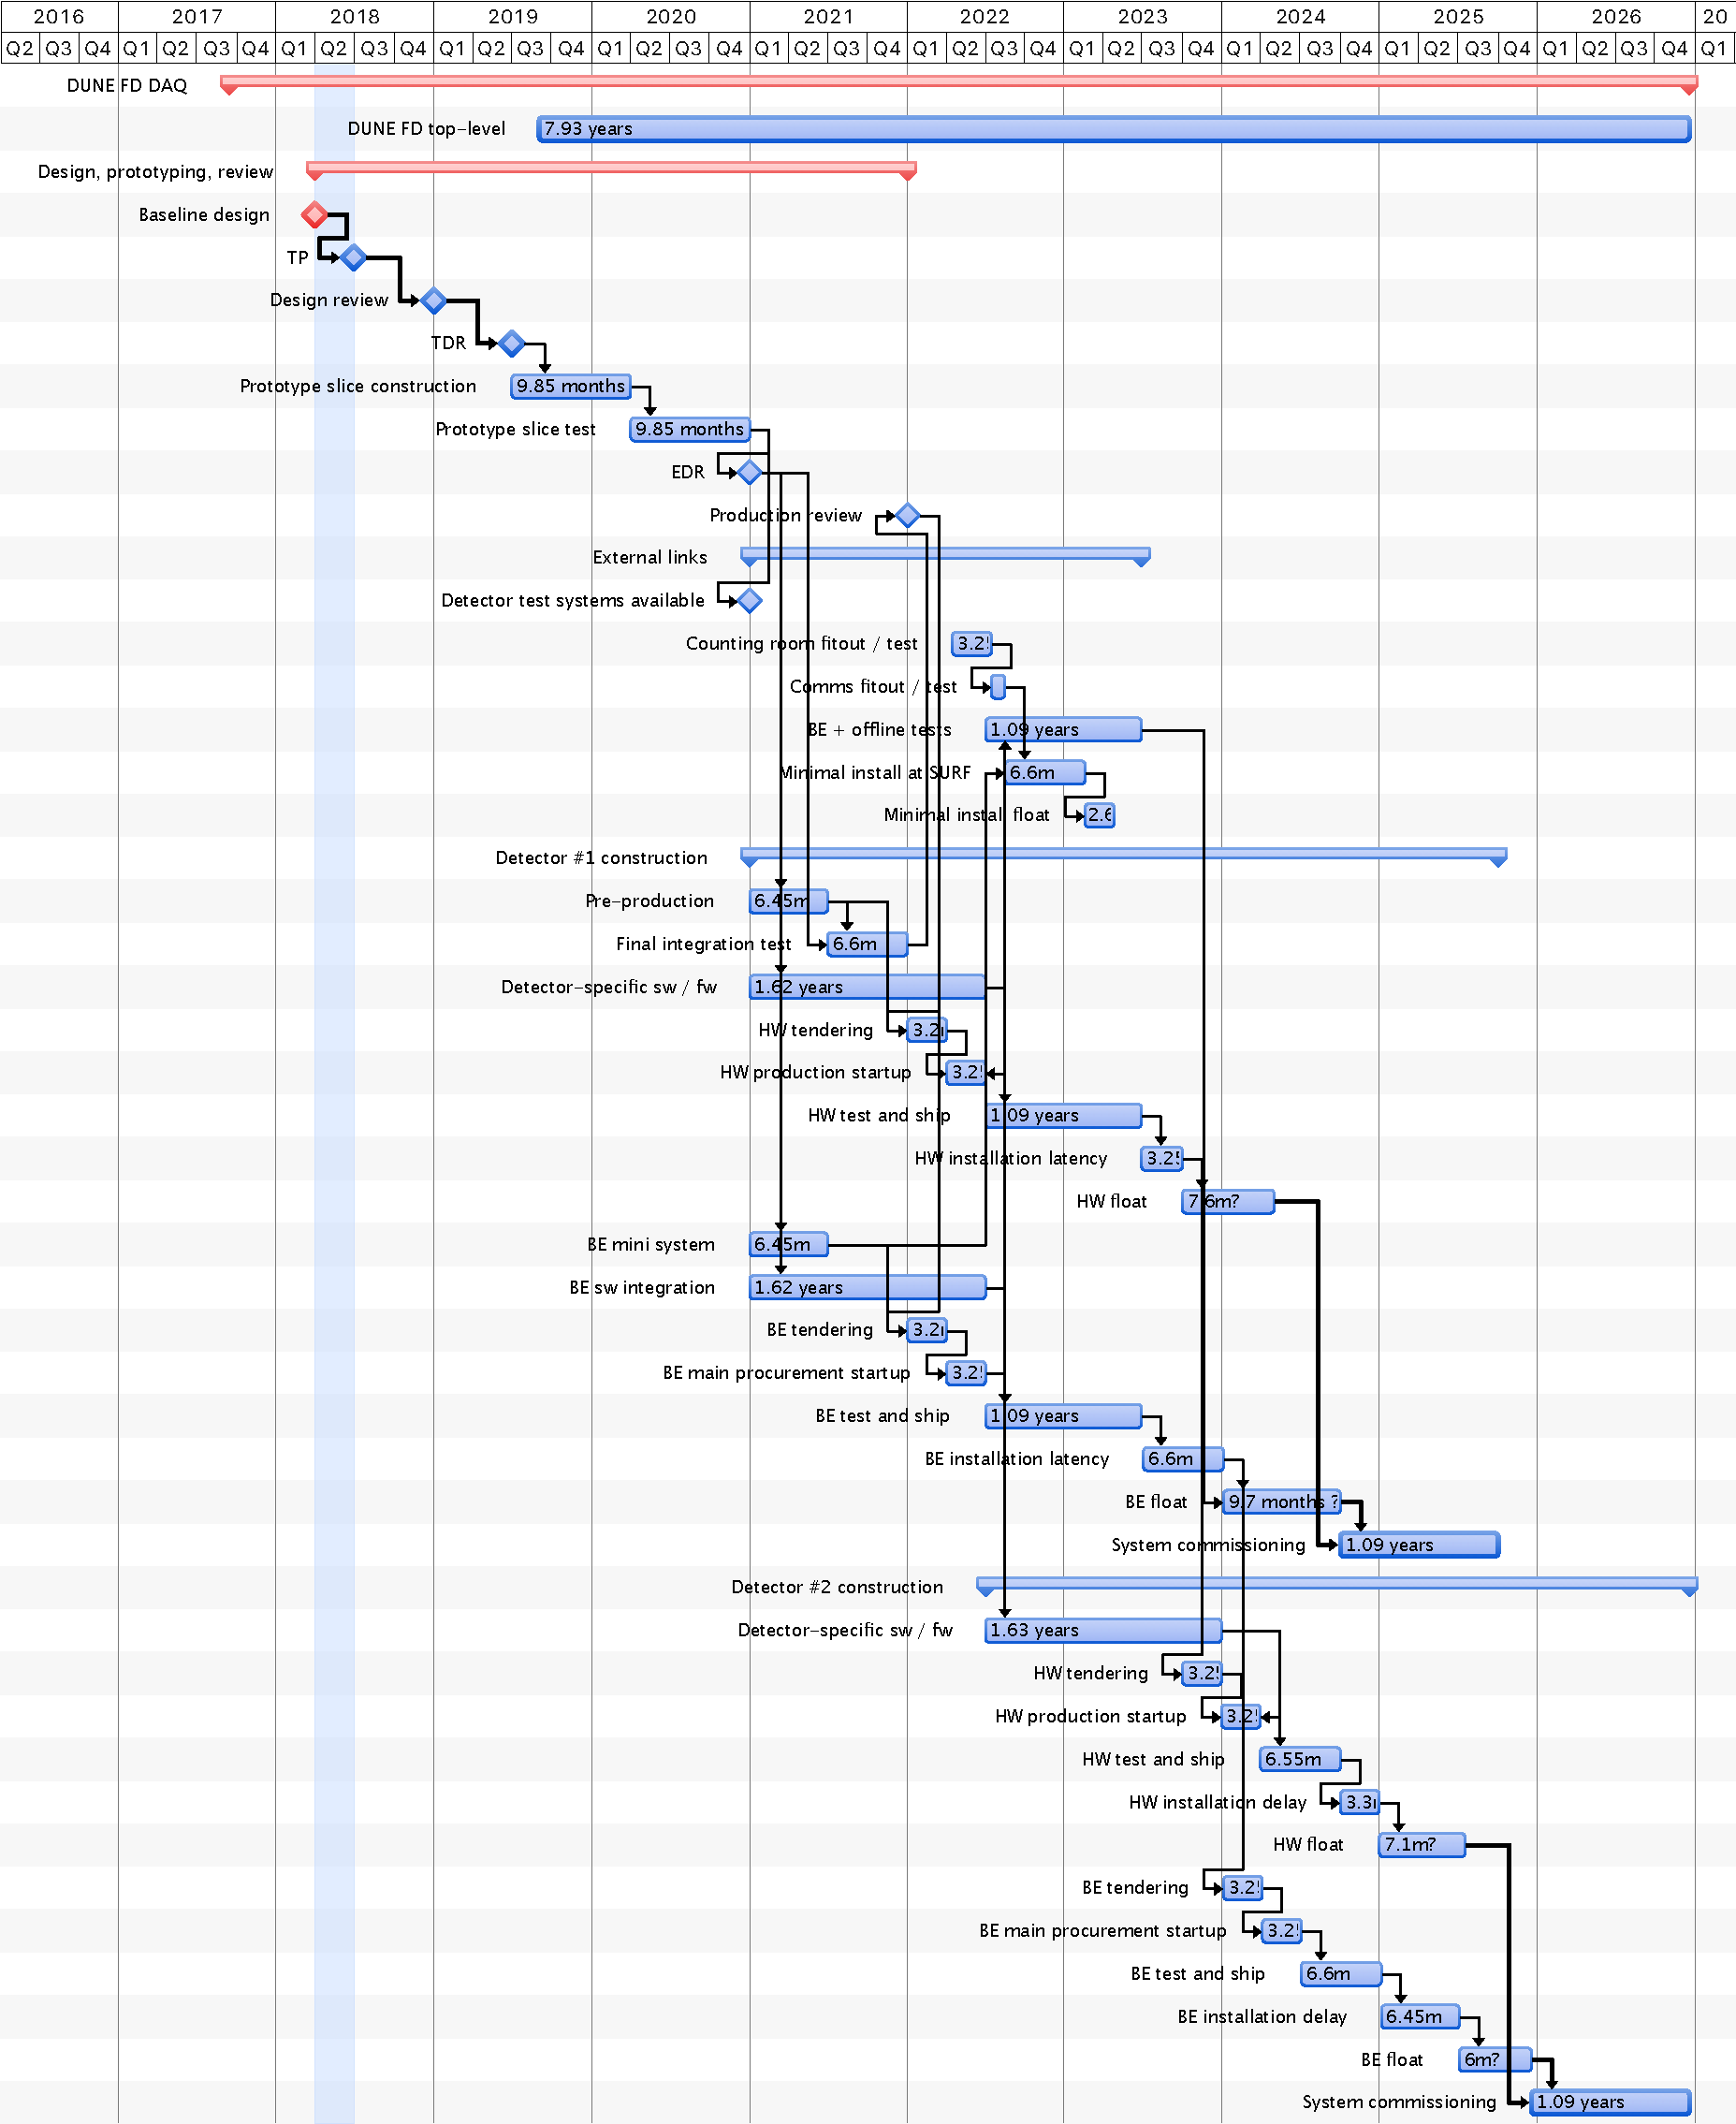
\includegraphics[width=0.8\textwidth]{DAQ-schedule.pdf}
\end{dunefigure}

A high-level breakdown of the DAQ cost for the first two detectors is summarised in Tab.~\ref{tab:daq-cost}.

\begin{dunetable}[DAQ high-level cost breakdown (2017 kUSD)]{lllll}{tab:daq-cost}{DAQ high-level cost breakdown}
	Cost item &  Module 1 & Module 2 & Common costs & Total \\ \toprowrule
	Data links & 741 & 133 & 0 & 874 \\
	Front-end hardware & 5110 & 0 & 0 & 5110 \\
	Front-end computing & 1029 & 710 & 0 & 1739 \\
	Back-end computing & 151 & 56 & 122 & 329 \\
	Service computing & 45 & 45 & 6 & 96 \\
	Timing system & 96 & 61 & 24 & 181 \\
	Network & 103 & 343 & 5 & 451 \\
	Infrastructure & 106 & 106 & 145 & 357 \\
	\bf{Total} & 7380 & 1454 & 303 & \bf{9136} \\
\end{dunetable}
